%DIF 1c1
%DIF LATEXDIFF DIFFERENCE FILE
%DIF DEL submitted/zscaling.tex   Tue May  5 13:18:46 2020
%DIF ADD zscaling.tex             Mon May  4 22:16:10 2020
%DIF < \documentclass[10pt,showpacs,showkeys,twocolumn]{revtex4}
%DIF -------
\documentclass[10pt,showpacs,showkeys,twocolumn]{revtex4-1} %DIF > 
%DIF -------
%%%%%%%%%%%%%%%%%%%%%%%%%%%%%%%%%%%%%%%%%%%%%%%%%%%%%%%%%%%%%%%%%%%%%%%%
% \usepackage[T1]{fontspec}
\usepackage{bm}
\usepackage{amssymb}
\usepackage{amsmath}
\usepackage{graphicx}
\usepackage{multirow}
%DIF 9d9
%DIF < \usepackage{float}
%DIF -------
\usepackage{MnSymbol}
%DIF 11d10
%DIF < \usepackage{comment}
%DIF -------
\usepackage{wasysym} 
\usepackage{stmaryrd}
\usepackage[outline]{contour}
\usepackage[dvipsnames]{xcolor}
%DIF 16a14
\usepackage{float} %DIF > 
%DIF -------

\definecolor{olive}{RGB}{182,187,37}
\usepackage[mathlines]{lineno}% Enable numbering of text and display math %DIF > 
%\linenumbers\relax % Commence numbering lines %DIF > 
%DIF PREAMBLE EXTENSION ADDED BY LATEXDIFF
%DIF UNDERLINE PREAMBLE %DIF PREAMBLE
\RequirePackage[normalem]{ulem} %DIF PREAMBLE
\RequirePackage{color}\definecolor{RED}{rgb}{1,0,0}\definecolor{BLUE}{rgb}{0,0,1} %DIF PREAMBLE
\providecommand{\DIFadd}[1]{{\protect\color{blue}\uwave{#1}}} %DIF PREAMBLE
\providecommand{\DIFdel}[1]{{\protect\color{red}\sout{#1}}}                      %DIF PREAMBLE
%DIF SAFE PREAMBLE %DIF PREAMBLE
\providecommand{\DIFaddbegin}{} %DIF PREAMBLE
\providecommand{\DIFaddend}{} %DIF PREAMBLE
\providecommand{\DIFdelbegin}{} %DIF PREAMBLE
\providecommand{\DIFdelend}{} %DIF PREAMBLE
%DIF FLOATSAFE PREAMBLE %DIF PREAMBLE
\providecommand{\DIFaddFL}[1]{\DIFadd{#1}} %DIF PREAMBLE
\providecommand{\DIFdelFL}[1]{\DIFdel{#1}} %DIF PREAMBLE
\providecommand{\DIFaddbeginFL}{} %DIF PREAMBLE
\providecommand{\DIFaddendFL}{} %DIF PREAMBLE
\providecommand{\DIFdelbeginFL}{} %DIF PREAMBLE
\providecommand{\DIFdelendFL}{} %DIF PREAMBLE
\newcommand{\DIFscaledelfig}{0.5}
%DIF HIGHLIGHTGRAPHICS PREAMBLE %DIF PREAMBLE
\RequirePackage{settobox} %DIF PREAMBLE
\RequirePackage{letltxmacro} %DIF PREAMBLE
\newsavebox{\DIFdelgraphicsbox} %DIF PREAMBLE
\newlength{\DIFdelgraphicswidth} %DIF PREAMBLE
\newlength{\DIFdelgraphicsheight} %DIF PREAMBLE
% store original definition of \includegraphics %DIF PREAMBLE
\LetLtxMacro{\DIFOincludegraphics}{\includegraphics} %DIF PREAMBLE
\newcommand{\DIFaddincludegraphics}[2][]{{\color{blue}\fbox{\DIFOincludegraphics[#1]{#2}}}} %DIF PREAMBLE
\newcommand{\DIFdelincludegraphics}[2][]{% %DIF PREAMBLE
\sbox{\DIFdelgraphicsbox}{\DIFOincludegraphics[#1]{#2}}% %DIF PREAMBLE
\settoboxwidth{\DIFdelgraphicswidth}{\DIFdelgraphicsbox} %DIF PREAMBLE
\settoboxtotalheight{\DIFdelgraphicsheight}{\DIFdelgraphicsbox} %DIF PREAMBLE
\scalebox{\DIFscaledelfig}{% %DIF PREAMBLE
\parbox[b]{\DIFdelgraphicswidth}{\usebox{\DIFdelgraphicsbox}\\[-\baselineskip] \rule{\DIFdelgraphicswidth}{0em}}\llap{\resizebox{\DIFdelgraphicswidth}{\DIFdelgraphicsheight}{% %DIF PREAMBLE
\setlength{\unitlength}{\DIFdelgraphicswidth}% %DIF PREAMBLE
\begin{picture}(1,1)% %DIF PREAMBLE
\thicklines\linethickness{2pt} %DIF PREAMBLE
{\color[rgb]{1,0,0}\put(0,0){\framebox(1,1){}}}% %DIF PREAMBLE
{\color[rgb]{1,0,0}\put(0,0){\line( 1,1){1}}}% %DIF PREAMBLE
{\color[rgb]{1,0,0}\put(0,1){\line(1,-1){1}}}% %DIF PREAMBLE
\end{picture}% %DIF PREAMBLE
}\hspace*{3pt}}} %DIF PREAMBLE
} %DIF PREAMBLE
\LetLtxMacro{\DIFOaddbegin}{\DIFaddbegin} %DIF PREAMBLE
\LetLtxMacro{\DIFOaddend}{\DIFaddend} %DIF PREAMBLE
\LetLtxMacro{\DIFOdelbegin}{\DIFdelbegin} %DIF PREAMBLE
\LetLtxMacro{\DIFOdelend}{\DIFdelend} %DIF PREAMBLE
\DeclareRobustCommand{\DIFaddbegin}{\DIFOaddbegin \let\includegraphics\DIFaddincludegraphics} %DIF PREAMBLE
\DeclareRobustCommand{\DIFaddend}{\DIFOaddend \let\includegraphics\DIFOincludegraphics} %DIF PREAMBLE
\DeclareRobustCommand{\DIFdelbegin}{\DIFOdelbegin \let\includegraphics\DIFdelincludegraphics} %DIF PREAMBLE
\DeclareRobustCommand{\DIFdelend}{\DIFOaddend \let\includegraphics\DIFOincludegraphics} %DIF PREAMBLE
\LetLtxMacro{\DIFOaddbeginFL}{\DIFaddbeginFL} %DIF PREAMBLE
\LetLtxMacro{\DIFOaddendFL}{\DIFaddendFL} %DIF PREAMBLE
\LetLtxMacro{\DIFOdelbeginFL}{\DIFdelbeginFL} %DIF PREAMBLE
\LetLtxMacro{\DIFOdelendFL}{\DIFdelendFL} %DIF PREAMBLE
\DeclareRobustCommand{\DIFaddbeginFL}{\DIFOaddbeginFL \let\includegraphics\DIFaddincludegraphics} %DIF PREAMBLE
\DeclareRobustCommand{\DIFaddendFL}{\DIFOaddendFL \let\includegraphics\DIFOincludegraphics} %DIF PREAMBLE
\DeclareRobustCommand{\DIFdelbeginFL}{\DIFOdelbeginFL \let\includegraphics\DIFdelincludegraphics} %DIF PREAMBLE
\DeclareRobustCommand{\DIFdelendFL}{\DIFOaddendFL \let\includegraphics\DIFOincludegraphics} %DIF PREAMBLE
%DIF END PREAMBLE EXTENSION ADDED BY LATEXDIFF

\begin{document}

\DIFdelbegin %DIFDELCMD < \title[Universal scaling for the ionization of biological molecules]{%%%
\DIFdelend \DIFaddbegin \title[General scaling rule for the ionization of biological molecules]{\DIFaddend 
\DIFdelbegin \DIFdel{Universal }\DIFdelend \DIFaddbegin \DIFadd{General }\DIFaddend scaling \DIFaddbegin \DIFadd{rule }\DIFaddend for the ionization of biological molecules \DIFaddbegin \\ \DIFaddend by 
highly charged ions}
\author{A. M. P. Mendez, C. C. Montanari, J. E. Miraglia}
\DIFdelbegin %DIFDELCMD < \affiliation{Instituto de Astronom\'{\i}a y F\'{\i}sica del Espacio 
%DIFDELCMD < (CONICET--UBA), \\ Buenos Aires, Argentina.}
%DIFDELCMD < %%%
\DIFdelend \DIFaddbegin \affiliation{Instituto de Astronom\'{\i}a y F\'{\i}sica del Espacio 
(CONICET-UBA), \\ Buenos Aires, Argentina.}
\DIFaddend 

\date{\DIFdelbegin %DIFDELCMD < \today%%%
\DIFdelend }% It is always \today, today,

\begin{abstract}
In the present work, we investigate scaling rules for the ionization 
cross sections of multicharged ions on molecules of biological interest. 
The cross sections are obtained \DIFdelbegin \DIFdel{from distorted--wave calculations for atomic targets combined with a stoichiometric model for the molecules proposed }\DIFdelend \DIFaddbegin \DIFadd{using a methodology presented }\DIFaddend in 
[Mendez \textit{et al.} J. Phys B (2020)]\DIFaddbegin \DIFadd{, which considers distorted-wave 
calculations for atomic targets combined with a molecular stoichiometric 
model}\DIFaddend . We examine ions with \DIFaddbegin \DIFadd{nuclear }\DIFaddend charges $Z$ from $+1$ to $+8$ 
\DIFdelbegin \DIFdel{in }\DIFdelend \DIFaddbegin \DIFadd{impacting on }\DIFaddend five nucleobases --adenine, cytosine, guanine, thymine, 
uracil--, tetrahydrofuran, pyrimidine, and \DIFdelbegin \DIFdel{also in }\DIFdelend water. We propose a scaling 
with the ion charge, which is valid in the intermediate to high energy 
range, i.e.\DIFaddbegin \DIFadd{, }\DIFaddend 0.2-5 MeV/amu for oxygen impact. We extend our work to a 
universal scaling for any ion and molecule, merging the forty 
\DIFdelbegin \DIFdel{ion--molecule }\DIFdelend \DIFaddbegin \DIFadd{ion-molecule }\DIFaddend systems analyzed here into a single band. Furthermore, our 
model proved to be valid for other molecules too.  
\end{abstract}

\keywords{ionization, scaling, molecules, charged-ions, DNA, 
multicharged ions}
\pacs{34.50Gb, 34.80Gs, 34.80Dp}

\maketitle
%\ioptwocol
\DIFaddbegin \linenumbers
\DIFaddend 

The ionization of biological molecules by multicharged ions has gained 
increasing interest due to medical and environmental 
\DIFdelbegin \DIFdel{reasons}\DIFdelend \DIFaddbegin \DIFadd{implementations}\DIFaddend ~\cite{PhysMed}, \DIFdelbegin \DIFdel{from }\DIFdelend \DIFaddbegin \DIFadd{which includes }\DIFaddend medical 
treatments~\cite{Mohamad2017,Solov2009,Denifl2011} \DIFdelbegin \DIFdel{to }\DIFdelend \DIFaddbegin \DIFadd{and }\DIFaddend contaminant 
recognition in biological materials~\cite{water,ferrazdias}. 
Many semiempirical \citep{vera_prl2013} and theoretical efforts are 
currently being undertaken~\DIFdelbegin \DIFdel{\mbox{%DIFAUXCMD
\cite{MendezJPB20,Quinto20,ludde2019,ludde2018,ludde2016,Champion2012} }\hspace{0pt}%DIFAUXCMD
}\DIFdelend \DIFaddbegin \DIFadd{\mbox{%DIFAUXCMD
\cite{MendezJPB20,Quinto20,ludde2019,ludde2018,
ludde2016,Champion2012} }\hspace{0pt}%DIFAUXCMD
}\DIFaddend to get reliable values for the ionization cross 
sections of these \DIFdelbegin \DIFdel{molecules}\DIFdelend \DIFaddbegin \DIFadd{molecular systems}\DIFaddend . 

\DIFdelbegin \DIFdel{Recently}\DIFdelend \DIFaddbegin \DIFadd{In recent work~\mbox{%DIFAUXCMD
\cite{MendezJPB20}}\hspace{0pt}%DIFAUXCMD
}\DIFaddend , we combined the \DIFdelbegin \DIFdel{continue distorted--wave }\DIFdelend \DIFaddbegin \DIFadd{continuum 
distorted-wave }\DIFaddend calculations (CDW) for atoms and the simple 
stoichiometric model (SSM), also known as the Bragg sum rule, to 
approximate the ionization cross sections of complex molecular targets 
by charged ions\DIFdelbegin \DIFdel{~\mbox{%DIFAUXCMD
\cite{MendezJPB20}}\hspace{0pt}%DIFAUXCMD
. The CDW--SSM approximation showed reasonable }\DIFdelend \DIFaddbegin \DIFadd{. The CDW-SSM approximation showed consistent }\DIFaddend results 
for over a hundred of \DIFdelbegin \DIFdel{ion--molecule }\DIFdelend \DIFaddbegin \DIFadd{ion-molecule }\DIFaddend systems. As expected, in the high 
energy range (i.e.\DIFaddbegin \DIFadd{, }\DIFaddend above 5 MeV/amu)\DIFaddbegin \DIFadd{, }\DIFaddend the ionization cross sections \DIFdelbegin \DIFdel{present }\DIFdelend \DIFaddbegin \DIFadd{of
the molecular systems follow }\DIFaddend the $Z^2$ dependence predicted by the 
first Born approximation. However, at intermediate energies, the 
dependence with $Z$ is \DIFdelbegin \DIFdel{more complex, and non--perturvative }\DIFdelend \DIFaddbegin \DIFadd{not straightforward since non-perturbative 
}\DIFaddend models are mandatory.

\DIFdelbegin \DIFdel{The intention of this letter is }\DIFdelend \DIFaddbegin \DIFadd{This letter intends }\DIFaddend to give a follow up of our previous work \DIFdelbegin \DIFdel{~\mbox{%DIFAUXCMD
\cite{MendezJPB20} }\hspace{0pt}%DIFAUXCMD
}\DIFdelend by 
proposing a scaling \DIFdelbegin \DIFdel{with the ion charge $Z$ of }\DIFdelend \DIFaddbegin \DIFadd{rule for }\DIFaddend the ionization cross sections of complex 
molecules \DIFdelbegin \DIFdel{, }\DIFdelend \DIFaddbegin \DIFadd{with the ion charge $Z$, which is }\DIFaddend valid at intermediate 
energies. In general, scaling rules are used as \DIFdelbegin \DIFdel{first--order tests }\DIFdelend \DIFaddbegin \DIFadd{first-order 
approximations }\DIFaddend in experimental measurements and multipurpose codes. 
\DIFdelbegin \DIFdel{Based on ~\mbox{%DIFAUXCMD
\cite{MendezJPB20}}\hspace{0pt}%DIFAUXCMD
, we propose a universal scaling for any ion--target system}\DIFdelend \DIFaddbegin \DIFadd{Furthermore, we explore the generality of our scaling rule by inspecting 
various other ion-target systems}\DIFaddend .

\DIFdelbegin \DIFdel{At intermediate impact energies, 
}\DIFdelend \DIFaddbegin \DIFadd{We have found in the literature two scaling rules applicable at 
intermediate impact energy range. The scaling rule suggested by }\DIFaddend Janev 
and Presnyakov~\cite{janev1980} \DIFdelbegin \DIFdel{suggest }\DIFdelend \DIFaddbegin \DIFadd{depends linearly with ion charge $Z$,
considering }\DIFaddend $\sigma/Z$ versus $E/Z$ \DIFdelbegin \DIFdel{as }\DIFdelend \DIFaddbegin \DIFadd{to be }\DIFaddend the \textit{natural} reduced 
form of the ionization cross section $\sigma$ and the incident ion 
energy $E$. \DIFdelbegin \DIFdel{Much more }\DIFdelend \DIFaddbegin \DIFadd{More }\DIFaddend recently, Montenegro and \DIFdelbegin \DIFdel{co--workers~\mbox{%DIFAUXCMD
\cite{dubois13,montenegro_pra13} }\hspace{0pt}%DIFAUXCMD
}\DIFdelend \DIFaddbegin \DIFadd{co-workers~\mbox{%DIFAUXCMD
\cite{dubois13,
montenegro_pra13} }\hspace{0pt}%DIFAUXCMD
}\DIFaddend proposed an alternative scaling by taking into account 
that \DIFdelbegin \DIFdel{$\sigma$ }\DIFdelend \DIFaddbegin \DIFadd{the cross section }\DIFaddend is a function of $Z^2/E$. Their scaling, given by 
\begin{equation}
    \sigma/Z^{\alpha}=f(E/Z^{2-\alpha}),
    \label{Montenegro}
\end{equation}
keeps the $Z^2/E$ relationship for any value of \DIFaddbegin \DIFadd{the parameter }\DIFaddend $\alpha$. 
In Ref.~\cite{dubois13}, the authors propose $\alpha=4/3$ for ionization 
of He and H$_2$ by \DIFdelbegin \DIFdel{different }\DIFdelend \DIFaddbegin \DIFadd{differently }\DIFaddend charged ions. 

\DIFdelbegin %DIFDELCMD < \begin{figure*}[!t]%%%
%DIF < [h]
%DIFDELCMD < \centering
%DIFDELCMD < 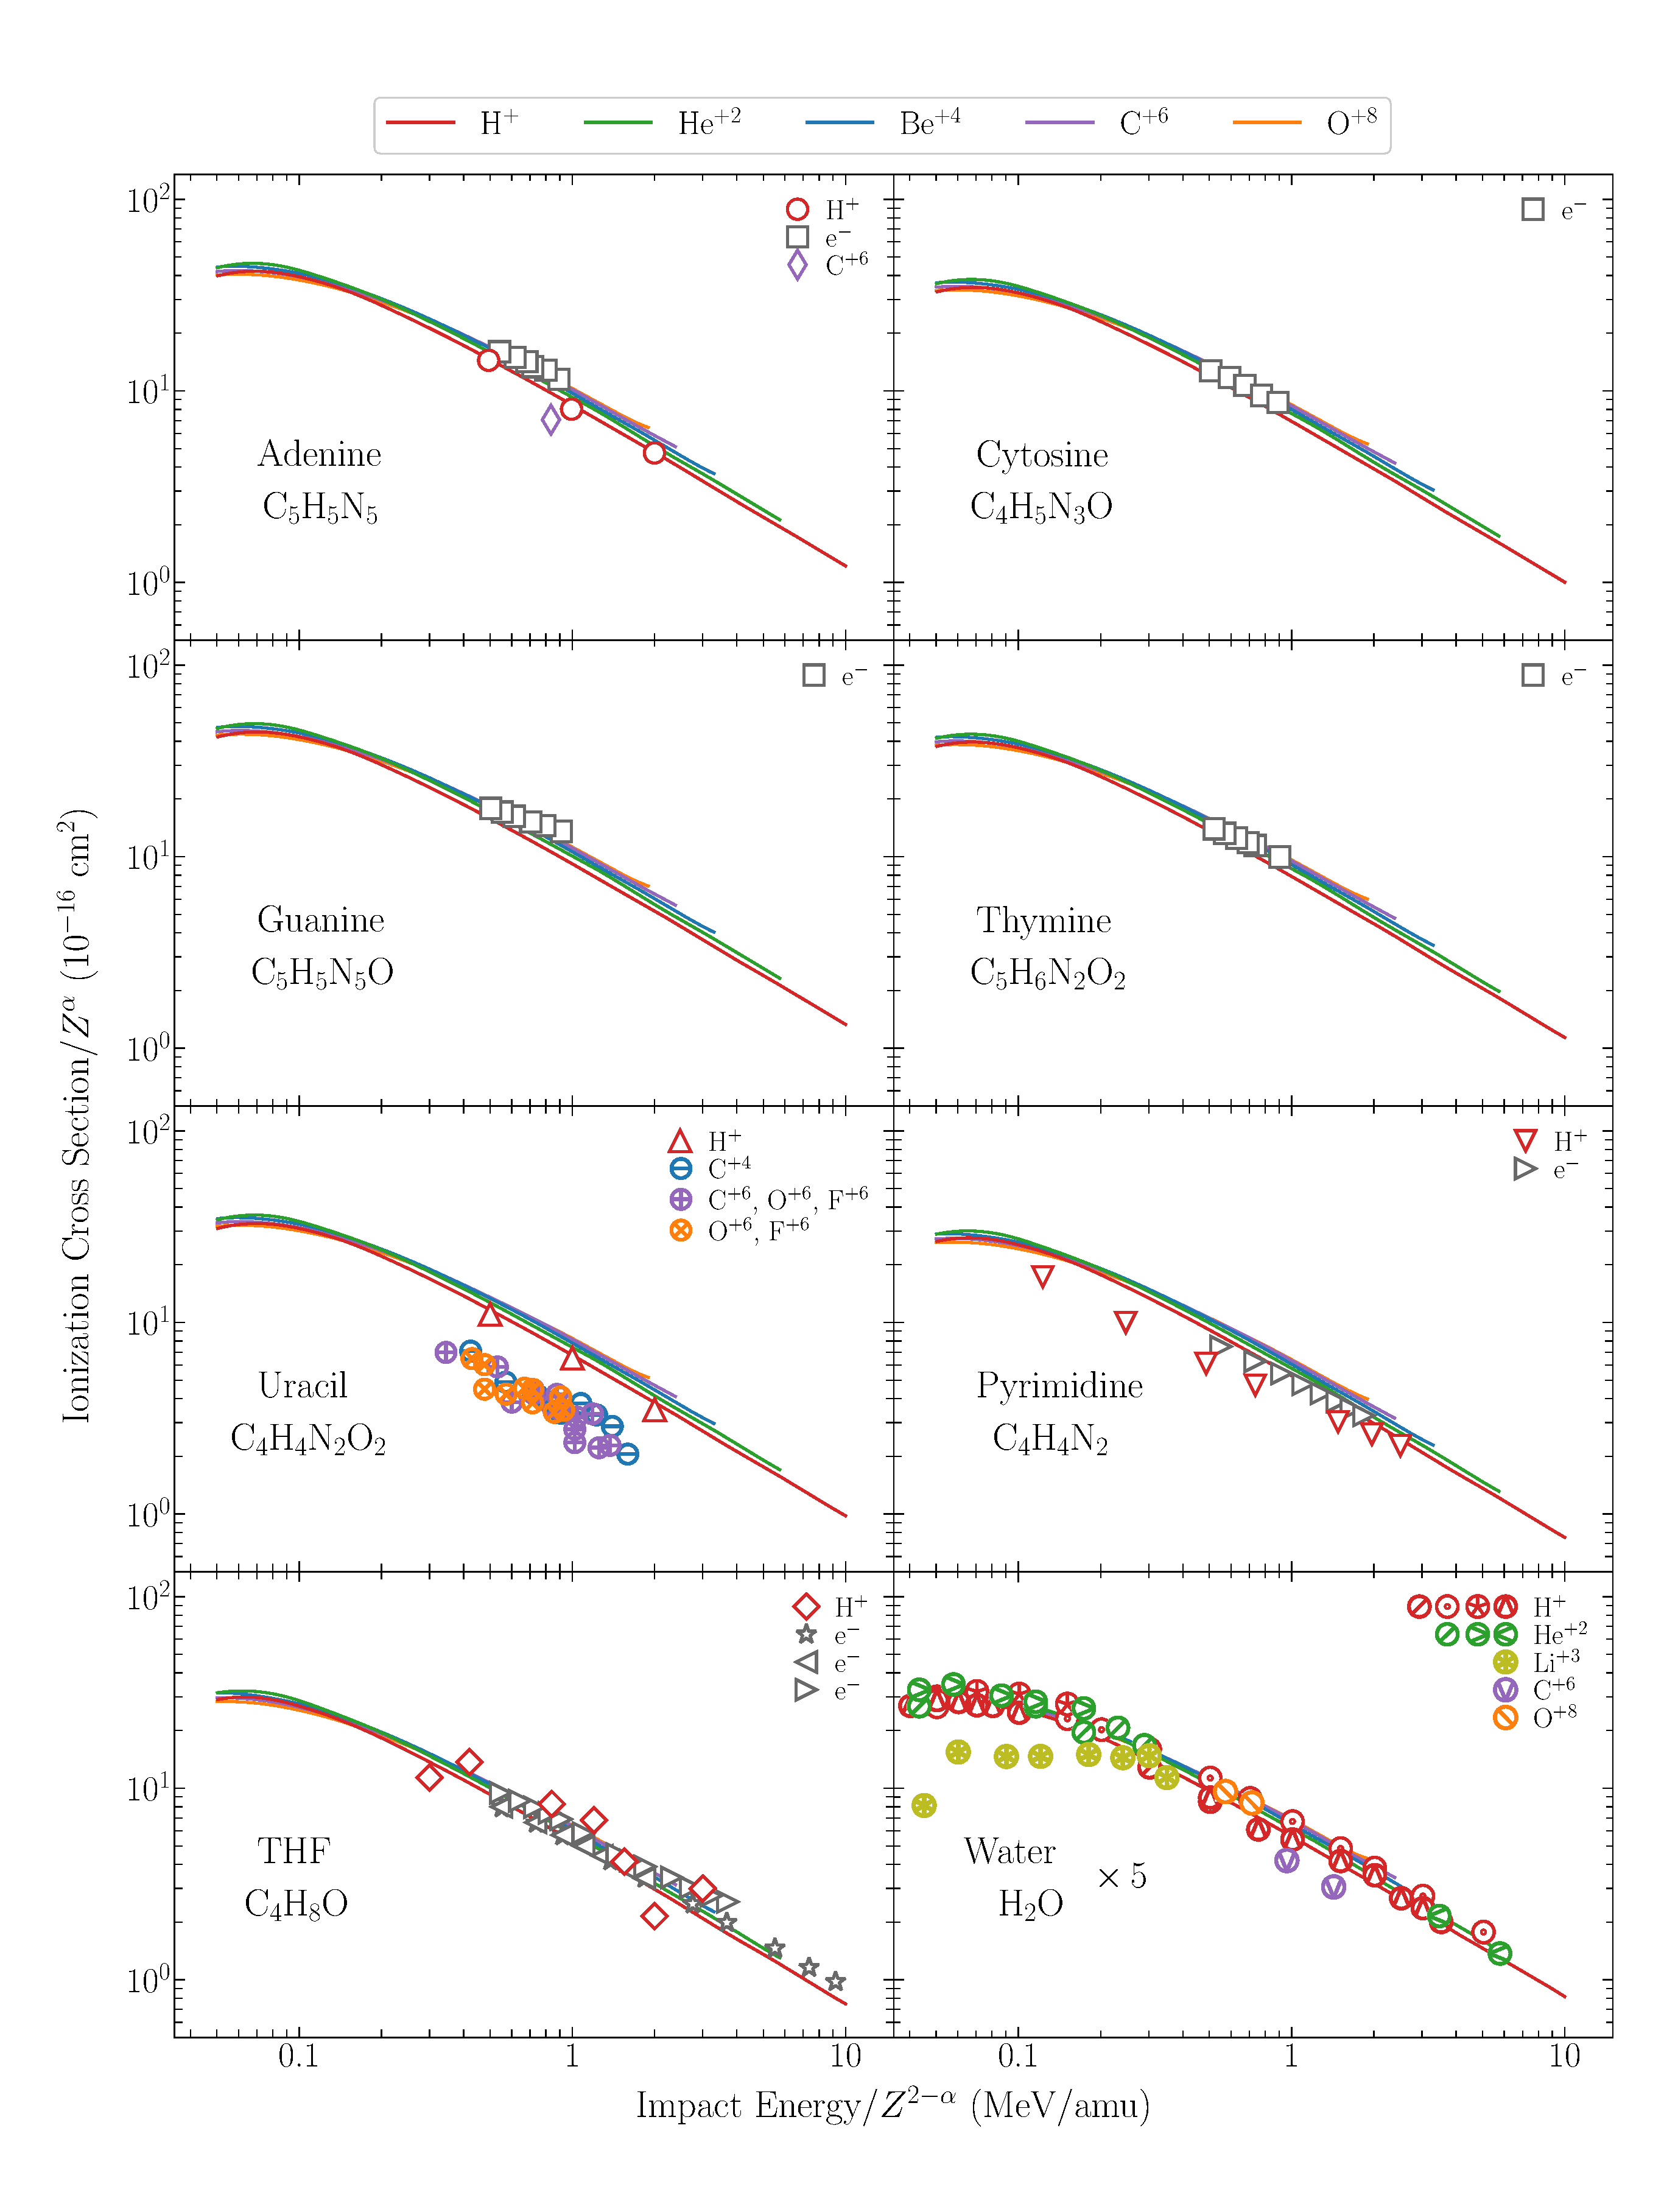
\includegraphics[width=0.7\textwidth]{zscale_alpha.eps}
%DIFDELCMD < %%%
%DIFDELCMD < \caption{%
{%DIFAUXCMD
\DIFdelFL{(Color online) Scaled ionization cross section $\sigma/Z^{\alpha}$ as a function of ion impact energy $E/Z^{2-\alpha}$ with $\alpha=1.2$. Colors are associated with the incident ion labeled on top of the figure. Curves: present CDW--SSM theoretical results. Symbols: experimental impact of 
\mbox{\LARGE$\color{red}\circ$} H$^+$~\mbox{%DIFAUXCMD
\cite{iriki2011} }\hspace{0pt}%DIFAUXCMD
and
}%DIFDELCMD < {\fontsize{11}{20}%%%
\DIFdelFL{$\color{Purple}\pmb{\lozenge}$}%DIFDELCMD < } %%%
\DIFdelFL{C$^{+6}$ \mbox{%DIFAUXCMD
\cite{tribedi2019} }\hspace{0pt}%DIFAUXCMD
on adenine;
H$^+$ on }%DIFDELCMD < {\fontsize{11}{20}%%%
\DIFdelFL{$\color{red}\pmb{\triangle}$}%DIFDELCMD < } %%%
\DIFdelFL{uracil~\mbox{%DIFAUXCMD
\cite{itoh2013}}\hspace{0pt}%DIFAUXCMD
, 
}%DIFDELCMD < {\fontsize{11}{20}%%%
\DIFdelFL{$\color{NavyBlue}\pmb{\ominus}$}%DIFDELCMD < } %%%
\DIFdelFL{C$^{+4}$, 
}%DIFDELCMD < {\fontsize{11}{20}%%%
\DIFdelFL{$\color{Purple}\pmb{\oplus}$}%DIFDELCMD < } %%%
\DIFdelFL{C$^{+6}$, O$^{+6}$, F$^{+6}$, and 
}%DIFDELCMD < {\fontsize{11}{20}%%%
\DIFdelFL{$\color{BurntOrange}\pmb{\otimes}$}%DIFDELCMD < } %%%
\DIFdelFL{O$^{+8}$, F$^{+8}$ on uracil~\mbox{%DIFAUXCMD
\cite{agnihotri2012,agnihotri2013}}\hspace{0pt}%DIFAUXCMD
;
H$^+$ on }%DIFDELCMD < {\fontsize{11}{20}%%%
\DIFdelFL{$\color{red}\pmb{\triangledown}$}%DIFDELCMD < } %%%
\DIFdelFL{pyrimidine~\mbox{%DIFAUXCMD
\cite{wolff2014}}\hspace{0pt}%DIFAUXCMD
, and
}%DIFDELCMD < {\fontsize{10}{20}%%%
\DIFdelFL{$\color{red}\pmb{\meddiamond}$}%DIFDELCMD < } %%%
\DIFdelFL{THF~\mbox{%DIFAUXCMD
\cite{wang2016}}\hspace{0pt}%DIFAUXCMD
;
%DIF <  water
\mbox{\fontsize{11}{20}$\color{red}\pmb{\odot}$}~\mbox{%DIFAUXCMD
\cite{Luna2007}}\hspace{0pt}%DIFAUXCMD
, 
}%DIFDELCMD < {\fontsize{11}{20}\color{red}%%%
\DIFdelFL{$\pmb{\logof}$}%DIFDELCMD < }%%%
\DIFdelFL{~\mbox{%DIFAUXCMD
\cite{Rudd86}}\hspace{0pt}%DIFAUXCMD
, 
}%DIFDELCMD < {\fontsize{11}{20}\color{red}%%%
\DIFdelFL{$\pmb{\varowedge}$}%DIFDELCMD < }%%%
\DIFdelFL{~\mbox{%DIFAUXCMD
\cite{pRudd85}}\hspace{0pt}%DIFAUXCMD
, 
}%DIFDELCMD < {\fontsize{11}{20}\color{red}%%%
\DIFdelFL{$\pmb{\varoslash}$}%DIFDELCMD < }%%%
\DIFdelFL{~\mbox{%DIFAUXCMD
\cite{toburen80} }\hspace{0pt}%DIFAUXCMD
H$^+$,
}%DIFDELCMD < {\fontsize{11}{20}\color{ForestGreen}%%%
\DIFdelFL{$\pmb{\varolessthan}$}%DIFDELCMD < }%%%
\DIFdelFL{~\mbox{%DIFAUXCMD
\cite{Ohsawa05}}\hspace{0pt}%DIFAUXCMD
,
}%DIFDELCMD < {\fontsize{11}{20}\color{ForestGreen}%%%
\DIFdelFL{$\pmb{\varogreaterthan}$}%DIFDELCMD < }%%%
\DIFdelFL{~\mbox{%DIFAUXCMD
\cite{Rudd85}}\hspace{0pt}%DIFAUXCMD
,
}%DIFDELCMD < {\fontsize{11}{20}\color{ForestGreen}%%%
\DIFdelFL{$\pmb{\varoslash}$}%DIFDELCMD < }%%%
\DIFdelFL{~\mbox{%DIFAUXCMD
\cite{toburen80} }\hspace{0pt}%DIFAUXCMD
He$^{+2}$,
}%DIFDELCMD < {\fontsize{11}{20}\color{Purple}%%%
\DIFdelFL{$\pmb{\ovee}$}%DIFDELCMD < }%%%
\DIFdelFL{~C$^{+6}$ \mbox{%DIFAUXCMD
\cite{DalCappello2009,Bhattacharjee17}}\hspace{0pt}%DIFAUXCMD
, and 
}%DIFDELCMD < {\fontsize{11}{20}\color{BurntOrange}%%%
\DIFdelFL{$\pmb{\obslash}$}%DIFDELCMD < }
%DIFDELCMD < %%%
\DIFdelFL{O$^{+8}$ \mbox{%DIFAUXCMD
\cite{Tribedi_O_water} }\hspace{0pt}%DIFAUXCMD
on water.
Markers~$\square$~\mbox{%DIFAUXCMD
\cite{rahman2016}}\hspace{0pt}%DIFAUXCMD
, 
$\rhd$~\mbox{%DIFAUXCMD
\cite{bug2017}}\hspace{0pt}%DIFAUXCMD
, 
$\lhd$~\mbox{%DIFAUXCMD
\cite{wolf2019}}\hspace{0pt}%DIFAUXCMD
, and 
$\medstar$~\mbox{%DIFAUXCMD
\cite{fuss2009} }\hspace{0pt}%DIFAUXCMD
correspond to electron impact ionization with the equi-velocity conversion.}}
%DIFAUXCMD
%DIFDELCMD < \label{fig:zreduced}
%DIFDELCMD < \end{figure*} 
%DIFDELCMD <  

%DIFDELCMD < %%%
\DIFdelend Combining our recent \DIFdelbegin \DIFdel{CDW--SSM }\DIFdelend \DIFaddbegin \DIFadd{CDW-SSM }\DIFaddend results~\cite{MendezJPB20} and 
Eq.~(\ref{Montenegro}), we propose here a $Z$-scaling and implement it 
for forty collisional systems. The \DIFdelbegin \DIFdel{ion--molecule }\DIFdelend \DIFaddbegin \DIFadd{ion-molecule }\DIFaddend systems are composed of 
eight targets: the DNA and RNA nucleobases --adenine, cytosine, guanine, 
thymine, uracil--, tetrahydrofuran (THF), pyrimidine, and water; and 
five \DIFdelbegin \DIFdel{charged ions}\DIFdelend \DIFaddbegin \DIFadd{ion species}\DIFaddend : H$^+$, He$^{+2}$, Be$^{+4}$, C$^{+6}$, and O$^{+8}$. 
We considered these systems as a benchmark for the present scaling. 

We found that the parameter $\alpha$ from Eq.~(\ref{Montenegro}) that 
fits the \DIFdelbegin \DIFdel{CDW--SSM }\DIFdelend \DIFaddbegin \DIFadd{CDW-SSM }\DIFaddend scaled cross sections for all the ions is $\alpha=1.2$. 
The validity of the theoretical scaling with the ion charge is \DIFdelbegin \DIFdel{very clear }\DIFdelend \DIFaddbegin \DIFadd{evident
}\DIFaddend in Fig.~\ref{fig:zreduced}, where the CDW-SSM curves \DIFdelbegin \DIFdel{lays }\DIFdelend \DIFaddbegin \DIFadd{lay }\DIFaddend one over the 
other. Our theoretical results are valid for impact energies around and 
above the maximum of the cross sections, which \DIFdelbegin \DIFdel{means above }\DIFdelend \DIFaddbegin \DIFadd{corresponds to an impact
energy range from }\DIFaddend 50 keV for \DIFdelbegin \DIFdel{impact of }\DIFdelend H$^+$ to 250 keV/amu for \DIFdelbegin \DIFdel{impact of }\DIFdelend O$^{+8}$. 

The scaling was tested with the experimental data available \DIFdelbegin \DIFdel{by impact of different charged ions \mbox{%DIFAUXCMD
\cite{itoh2013,iriki2011,wolff2014,wang2016,tribedi2019,agnihotri2012,agnihotri2013,Luna2007,Rudd86,Rudd85,Luna_Li_water,DalCappello2009,Tribedi_O_water}}\hspace{0pt}%DIFAUXCMD
}\DIFdelend \DIFaddbegin \DIFadd{for 
ionization by the impact of differently charged ions \mbox{%DIFAUXCMD
\cite{itoh2013,
iriki2011,wolff2014,wang2016,tribedi2019,agnihotri2012,agnihotri2013,
Luna2007,Rudd86,Rudd85,Luna_Li_water,DalCappello2009,Tribedi_O_water}}\hspace{0pt}%DIFAUXCMD
}\DIFaddend , 
and also by electron impact at sufficiently high velocity 
\cite{rahman2016,bug2017,wolf2019,fuss2009}. As can be noted, most of 
the data in Fig.~\ref{fig:zreduced} \DIFdelbegin \DIFdel{confirms }\DIFdelend \DIFaddbegin \DIFadd{confirm }\DIFaddend the present scaling, even 
for O$^{+8}$ in water~\cite{Tribedi_O_water}. However, the data of 
uracil by swift C, O\DIFaddbegin \DIFadd{, }\DIFaddend and F ions in \cite{agnihotri2012,agnihotri2013} 
are too low compared with our \DIFdelbegin \DIFdel{CDW--SSM }\DIFdelend \DIFaddbegin \DIFadd{CDW-SSM }\DIFaddend results, but also as compared 
with Itoh \textit{et al.} data \cite{itoh2013}, and with the CTMC 
calculations by Sarkadi\DIFaddbegin \DIFadd{~}\DIFaddend \cite{sarkadi2016}. The data for Li$^{+3}$ in 
water from Ref.~\cite{Luna_Li_water} also spreads out from the present 
theoretical curves for $E<600$ keV/amu.

The good results obtained in the scaling with the ion charge challenged 
us to look for a more general scaling rule that could predict values 
for ionization cross sections of any ion in any molecule. To that end, 
we resorted to the number of active electrons in each atom $n_e$ 
proposed in \cite{MendezJPB20}, and combined it with the $Z$-scaling 
displayed in Fig.~\ref{fig:zreduced}.


\DIFaddbegin \begin{figure*}[!htb]
\centering
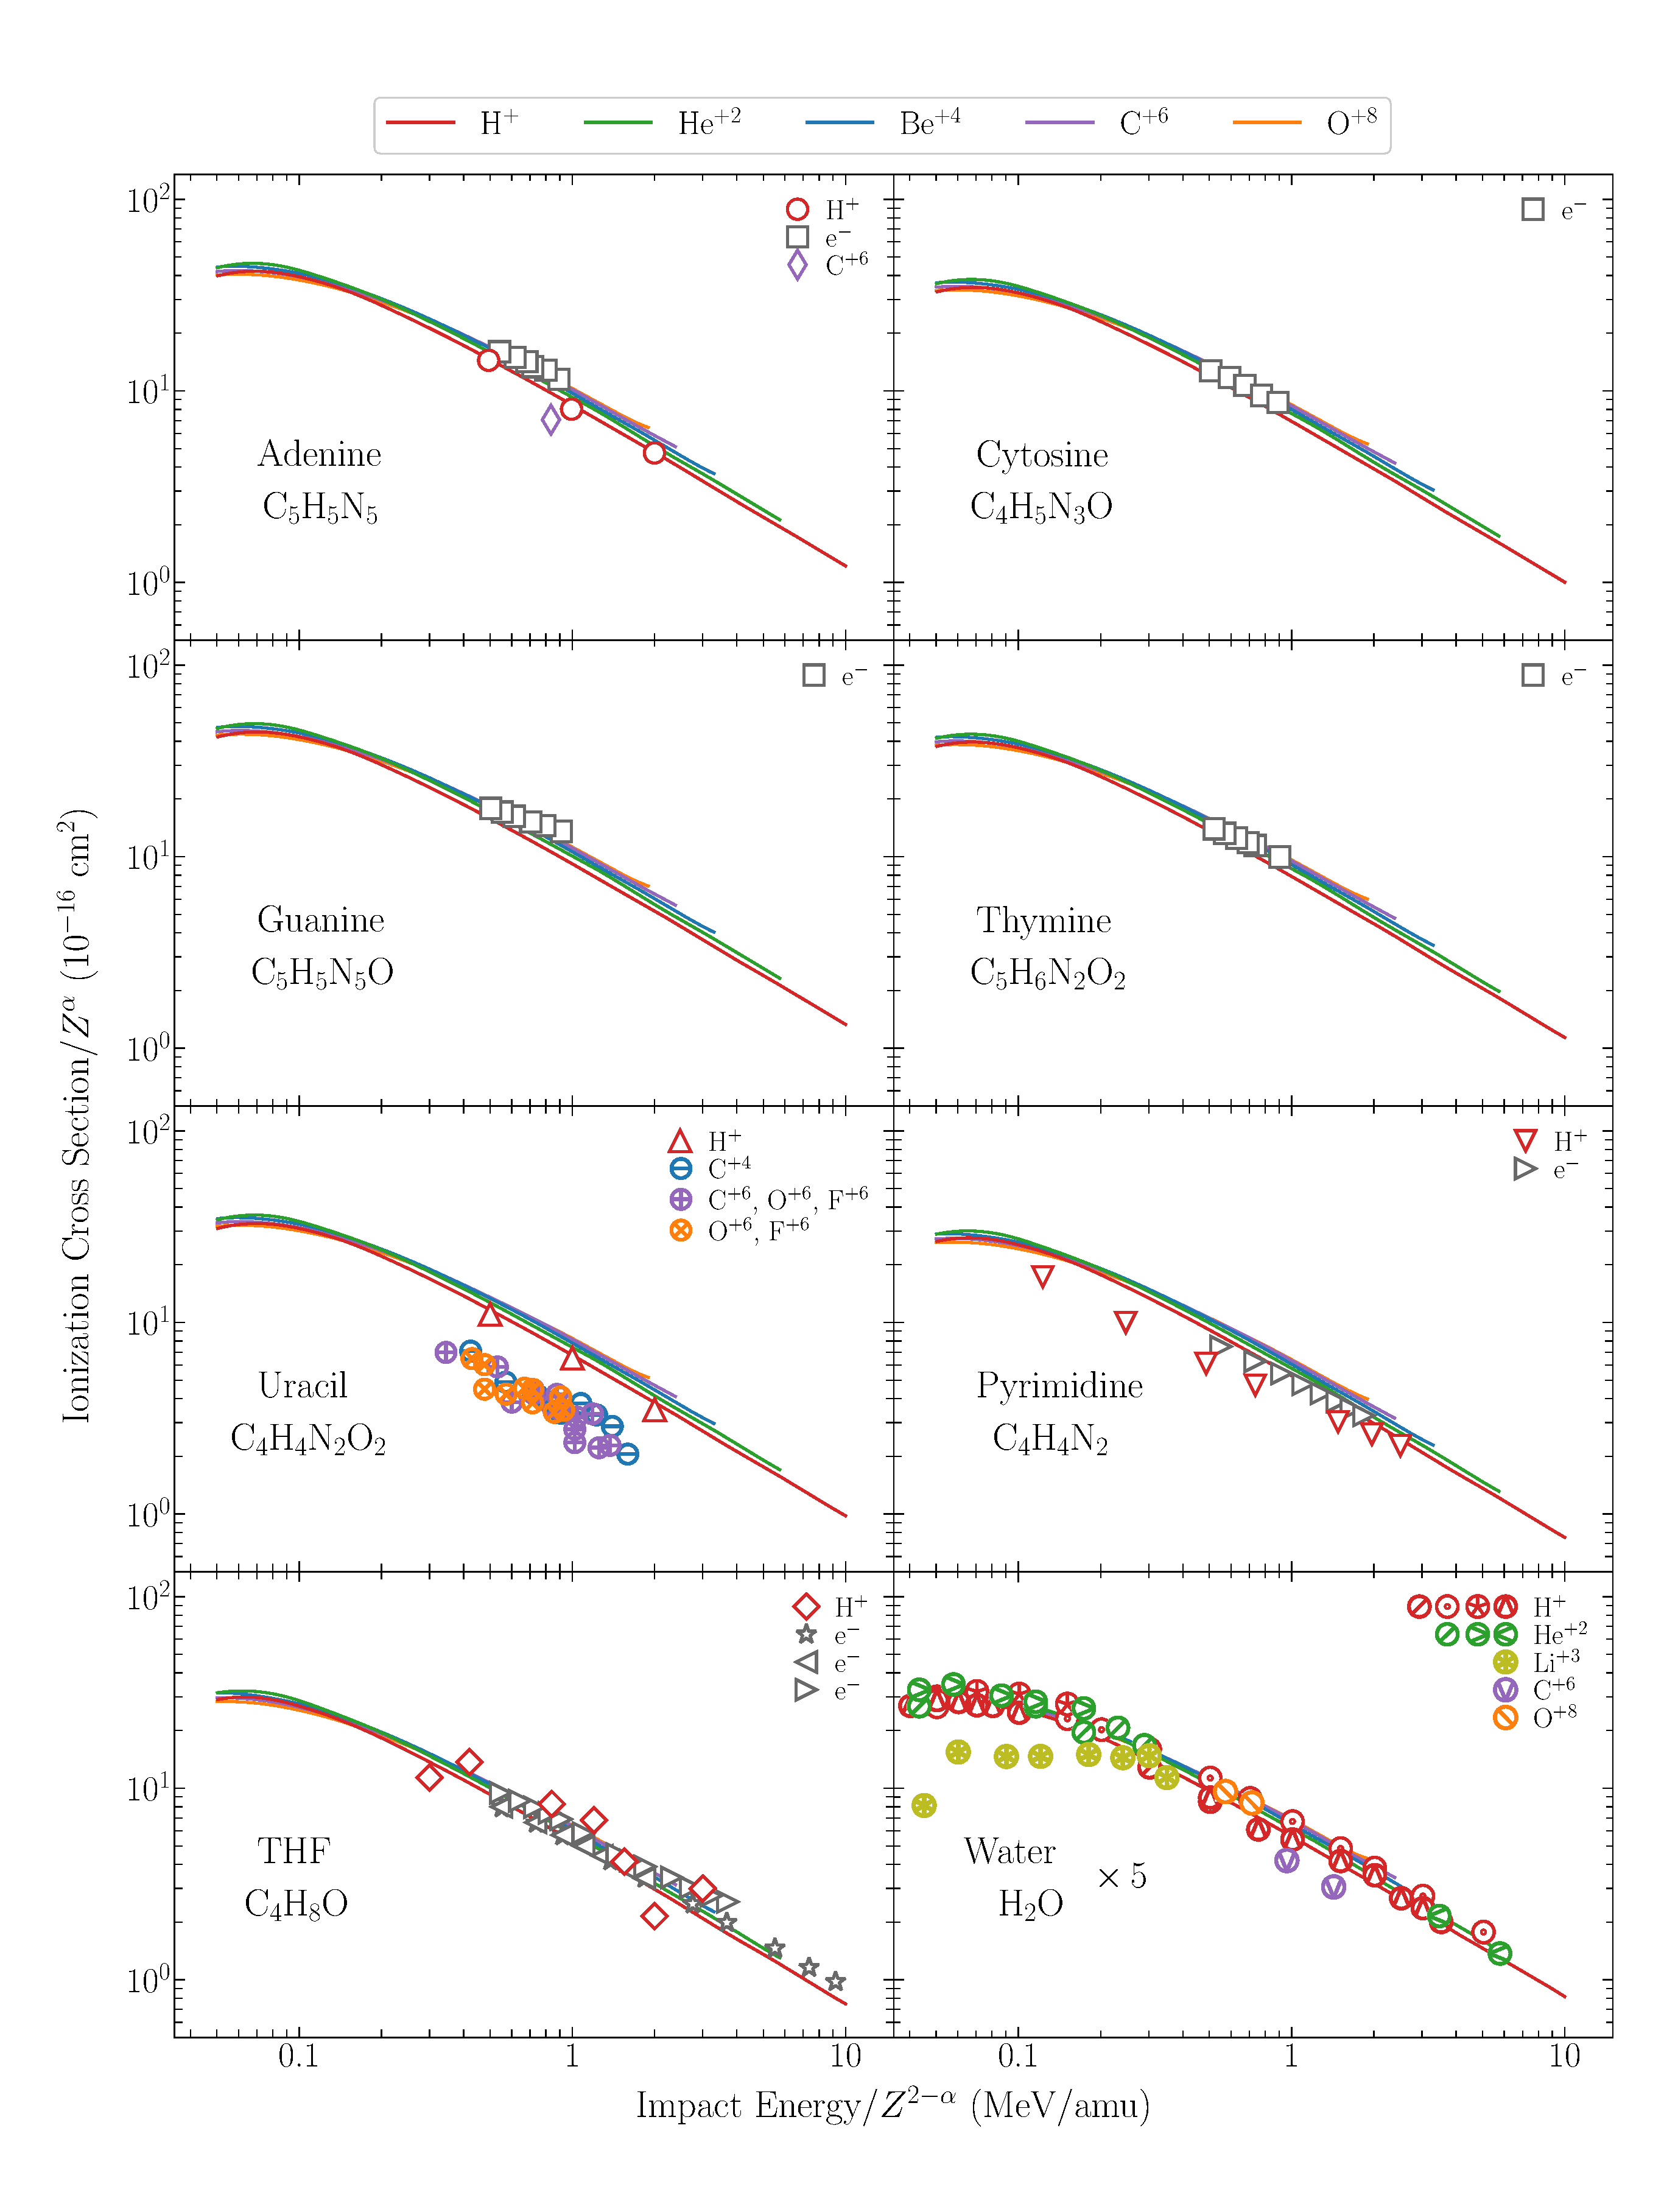
\includegraphics[width=0.9\textwidth]{zscale_alpha.eps}
\caption{\DIFaddFL{(Color online) Scaled ionization cross section $\sigma/Z^{\alpha}$ 
as a function of ion impact energy $E/Z^{2-\alpha}$ with $\alpha=1.2$. 
Colors are associated with the incident ion labeled on top of the figure. 
Curves: present CDW-SSM theoretical results. Symbols: experimental 
impact of \mbox{\LARGE$\color{red}\circ$} H$^+$~\mbox{%DIFAUXCMD
\cite{iriki2011} }\hspace{0pt}%DIFAUXCMD
and
}{\fontsize{11}{20}\DIFaddFL{$\color{Purple}\pmb{\lozenge}$}} \DIFaddFL{C$^{+6}$ 
\mbox{%DIFAUXCMD
\cite{tribedi2019} }\hspace{0pt}%DIFAUXCMD
on adenine;
H$^+$ on }{\fontsize{11}{20}\DIFaddFL{$\color{red}\pmb{\triangle}$}} \DIFaddFL{uracil~\mbox{%DIFAUXCMD
\cite{itoh2013}}\hspace{0pt}%DIFAUXCMD
, 
}{\fontsize{11}{20}\DIFaddFL{$\color{NavyBlue}\pmb{\ominus}$}} \DIFaddFL{C$^{+4}$, 
}{\fontsize{11}{20}\DIFaddFL{$\color{Purple}\pmb{\oplus}$}} \DIFaddFL{C$^{+6}$, O$^{+6}$, F$^{+6}$, and 
}{\fontsize{11}{20}\DIFaddFL{$\color{BurntOrange}\pmb{\otimes}$}} \DIFaddFL{O$^{+8}$, 
F$^{+8}$ on uracil~\mbox{%DIFAUXCMD
\cite{agnihotri2012,agnihotri2013}}\hspace{0pt}%DIFAUXCMD
;
H$^+$ on }{\fontsize{11}{20}\DIFaddFL{$\color{red}\pmb{\triangledown}$}} 
\DIFaddFL{pyrimidine~\mbox{%DIFAUXCMD
\cite{wolff2014}}\hspace{0pt}%DIFAUXCMD
, and 
}{\fontsize{10}{20}\DIFaddFL{$\color{red}\pmb{\meddiamond}$}} \DIFaddFL{THF~\mbox{%DIFAUXCMD
\cite{wang2016}}\hspace{0pt}%DIFAUXCMD
;
%DIF >  water
\mbox{\fontsize{11}{20}$\color{red}\pmb{\odot}$}~\mbox{%DIFAUXCMD
\cite{Luna2007}}\hspace{0pt}%DIFAUXCMD
, 
}{\fontsize{11}{20}\color{red}\DIFaddFL{$\pmb{\logof}$}}\DIFaddFL{~\mbox{%DIFAUXCMD
\cite{Rudd86}}\hspace{0pt}%DIFAUXCMD
, 
}{\fontsize{11}{20}\color{red}\DIFaddFL{$\pmb{\varowedge}$}}\DIFaddFL{~\mbox{%DIFAUXCMD
\cite{pRudd85}}\hspace{0pt}%DIFAUXCMD
, 
}{\fontsize{11}{20}\color{red}\DIFaddFL{$\pmb{\varoslash}$}}\DIFaddFL{~\mbox{%DIFAUXCMD
\cite{toburen80} }\hspace{0pt}%DIFAUXCMD
H$^+$,
}{\fontsize{11}{20}\color{ForestGreen}\DIFaddFL{$\pmb{\varolessthan}$}}\DIFaddFL{~\mbox{%DIFAUXCMD
\cite{Ohsawa05}}\hspace{0pt}%DIFAUXCMD
,
}{\fontsize{11}{20}\color{ForestGreen}\DIFaddFL{$\pmb{\varogreaterthan}$}}\DIFaddFL{~\mbox{%DIFAUXCMD
\cite{Rudd85}}\hspace{0pt}%DIFAUXCMD
,
}{\fontsize{11}{20}\color{ForestGreen}\DIFaddFL{$\pmb{\varoslash}$}}\DIFaddFL{~\mbox{%DIFAUXCMD
\cite{toburen80} }\hspace{0pt}%DIFAUXCMD
He$^{+2}$,
}{\fontsize{11}{20}\color{Purple}\DIFaddFL{$\pmb{\ovee}$}}\DIFaddFL{~C$^{+6}$ \mbox{%DIFAUXCMD
\cite{DalCappello2009,Bhattacharjee17}}\hspace{0pt}%DIFAUXCMD
, and 
}{\fontsize{11}{20}\color{BurntOrange}\DIFaddFL{$\pmb{\obslash}$}}
\DIFaddFL{O$^{+8}$ \mbox{%DIFAUXCMD
\cite{Tribedi_O_water} }\hspace{0pt}%DIFAUXCMD
on water.
Markers~$\square$~\mbox{%DIFAUXCMD
\cite{rahman2016}}\hspace{0pt}%DIFAUXCMD
, 
$\rhd$~\mbox{%DIFAUXCMD
\cite{bug2017}}\hspace{0pt}%DIFAUXCMD
, 
$\lhd$~\mbox{%DIFAUXCMD
\cite{wolf2019}}\hspace{0pt}%DIFAUXCMD
, and 
$\medstar$~\mbox{%DIFAUXCMD
\cite{fuss2009} }\hspace{0pt}%DIFAUXCMD
correspond to electron impact ionization with 
the equi-velocity conversion.}}
\label{fig:zreduced}
\end{figure*} 

\DIFaddend The CDW ionization cross sections $\sigma^{\mathrm{CDW}}$ of atomic H, 
C, N, O targets scale as $\sigma_e=\sigma^{\mathrm{CDW}}/n_e$ with $n_e$ 
being $1$ for H, $4$ for C, N, and O, i.e.\DIFaddbegin \DIFadd{,
}\DIFaddend \begin{equation}
 \frac{\sigma_{\mathrm{H}}^{\mathrm{CDW}}}{1}\sim
 \frac{\sigma_{\mathrm{C}}^{\mathrm{CDW}}}{4}\sim
 \frac{\sigma_{\mathrm{N}}^{\mathrm{CDW}}}{4}\sim
 \frac{\sigma_{\mathrm{O}}^{\mathrm{CDW}}}{4}
\end{equation}
The SSM leads to the molecular numbers of active electrons included in 
Table \ref{nn}.

\contourlength{0.03em}
\contournumber{30}

\DIFdelbegin %DIFDELCMD < \begin{table}[H]
%DIFDELCMD < %%%
\DIFdelendFL \DIFaddbeginFL \begin{table}[t]
\DIFaddendFL \begin{center}
\begin{tabular}{|ll|ll|ll|}
\hline
 Molecule & $n_e$ & Molecule          & $n_e$ & Molecule          & $n_e$ \\
\hline
 H$_2$O   & 6  & CO$_2$               \DIFdelbeginFL \DIFdelFL{\ \ \ \ }\DIFdelendFL & 12 & C$_4$H$_5$N$_3$O     \DIFdelbeginFL \DIFdelFL{\ \ \ \ }\DIFdelendFL & 37   \\ 
 N$_2$    & 8  & C$_4$H$_8$O          \DIFdelbeginFL \DIFdelFL{\ \ \ \ }\DIFdelendFL & 28 & C$_5$H$_6$N$_2$O$_2$ \DIFdelbeginFL \DIFdelFL{\ \ \ \ }\DIFdelendFL & 42   \\ 
 O$_2$    & 8  & C$_4$H$_4$N$_2$      \DIFdelbeginFL \DIFdelFL{\ \ \ \  }\DIFdelendFL & 28 & C$_5$H$_5$N$_5$      \DIFdelbeginFL \DIFdelFL{\ \ \ \ }\DIFdelendFL & 45   \\ 
 CH$_4$   & 8  & C$_4$H$_4$N$_2$O$_2$ \DIFdelbeginFL \DIFdelFL{\ \ \ \ }\DIFdelendFL & 36 & C$_5$H$_5$N$_5$O     \DIFdelbeginFL \DIFdelFL{\ \ \ \ }\DIFdelendFL & 49   \\ 
 \hline
\end{tabular}
\caption{Number of active electrons per target at intermediate to high 
energies obtained from the CDW calculations~\cite{MendezJPB20}.}
\label{nn}
\end{center}
\end{table}

\begin{figure*}[!t]%[h]
\centering
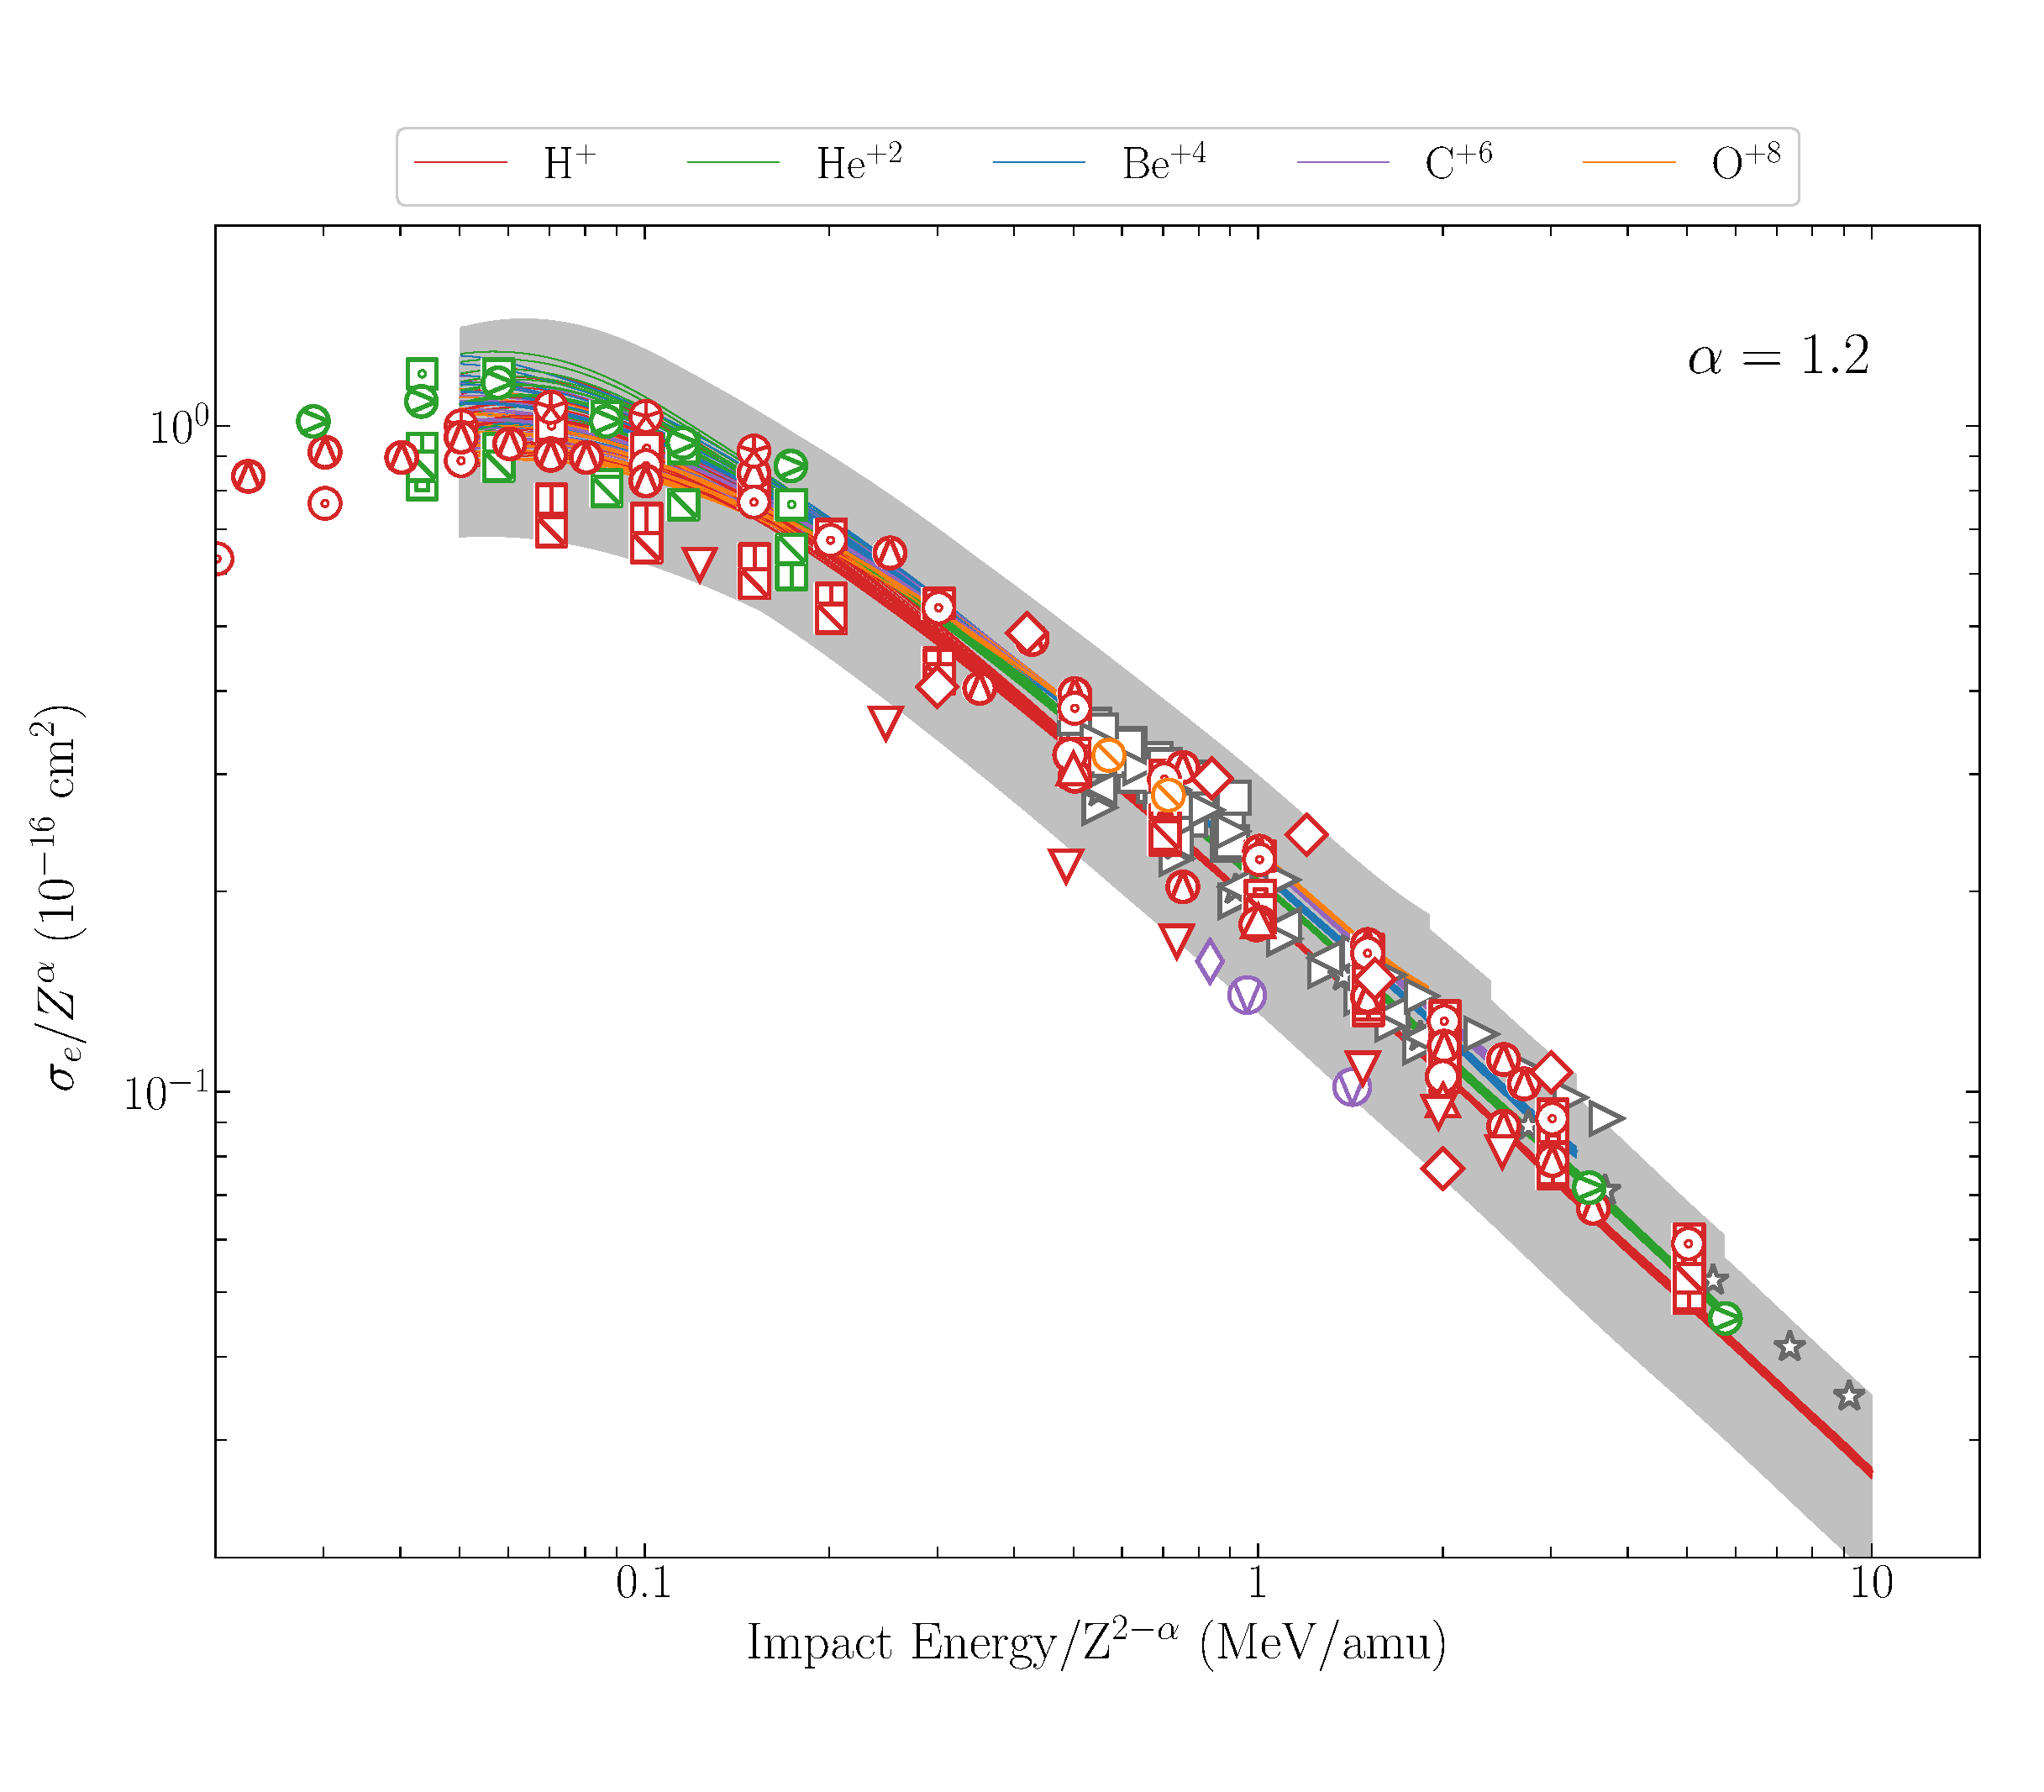
\includegraphics[width=0.7\textwidth]{zmol_werror.eps}
\caption{(Color online) Universal scaling with the ions charge $Z$ and 
the number of active electrons in the molecule $n_e$ given by Eq. 
(\ref{u-scaling}) \DIFaddbeginFL \DIFaddFL{with $\alpha=1.2$}\DIFaddendFL . Curves: present CDW-SSM theoretical 
results. Symbols: experimental impact of H$^+$ on 
\mbox{\LARGE$\color{red}\circ$} adenine~\cite{iriki2011}, 
{\fontsize{11}{20}$\color{red}\pmb{\triangle}$} uracil~\cite{itoh2013}, 
{\fontsize{11}{20}$\color{red}\pmb{\triangledown}$} pyrimidine~\cite{wolff2014} and 
{\fontsize{10}{20}$\color{red}\pmb{\meddiamond}$} THF~\cite{wang2016};
{\fontsize{11}{20}$\color{Purple}\pmb{\lozenge}$} C$^{+6}$ on adenine \cite{tribedi2019};
\mbox{\fontsize{11}{20}$\color{red}\pmb{\odot}$}~\cite{Luna2007}, 
{\fontsize{11}{20}\color{red}$\pmb{\logof}$}~\cite{Rudd86}, 
{\fontsize{11}{20}\color{red}$\pmb{\varowedge}$}~\cite{pRudd85}, 
{\fontsize{11}{20}\color{red}$\pmb{\varoslash}$}~\cite{toburen80} H$^+$,
{\fontsize{11}{20}\color{ForestGreen}$\pmb{\varolessthan}$}~\cite{Ohsawa05},
{\fontsize{11}{20}\color{ForestGreen}$\pmb{\varogreaterthan}$}~\cite{Rudd85},
{\fontsize{11}{20}\color{ForestGreen}$\pmb{\varoslash}$}~\cite{toburen80} He$^{+2}$,
{\fontsize{11}{20}\color{Purple}$\pmb{\ovee}$}~C$^{+6}$ \cite{DalCappello2009,Bhattacharjee17}, and 
{\fontsize{11}{20}\color{BurntOrange}$\pmb{\obslash}$}
O$^{+8}$ \cite{Tribedi_O_water} on water.
H$^{+}$ impact on 
{\fontsize{11}{20}${\color{red}\pmb{\boxast}}$}~N$_2$, 
{\fontsize{11}{20}${\color{red}\pmb{\boxbox}}$}~O$_2$, 
{\fontsize{11}{20}${\color{red}\pmb{\boxbar}}$}~CO, 
{\fontsize{11}{20}${\color{red}\pmb{\boxbslash}}$}~CO$_2$, and
{\fontsize{11}{20}${\color{red}\pmb{\boxdot}}$}~CH$_4$; 
and He$^{+2}$ impact on 
{\fontsize{11}{20}${\color{ForestGreen}\pmb{\boxast}}$}~N$_2$,
{\fontsize{11}{20}${\color{ForestGreen}\pmb{\boxbox}}$}~O$_2$, 
{\fontsize{11}{20}${\color{ForestGreen}\pmb{\boxbar}}$}~CO, 
{\fontsize{11}{20}${\color{ForestGreen}\pmb{\boxbslash}}$}~CO$_2$, and
{\fontsize{11}{20}${\color{ForestGreen}\pmb{\boxdot}}$} 
\DIFdelbeginFL \DIFdelFL{~}\DIFdelendFL CH$_4$~\cite{Rudd85,Rudd1983}, 
{\fontsize{11}{20}${\color{red}\pmb{\varowedge}}$}~H$^{+}$ on 
CH$_4$~\cite{Luna2019}; 
and electron impact on $\rhd$~pyrimidine~\cite{bug2017}, and $\lhd$, 
$\medstar$~\cite{wolf2019,fuss2009} THF.}
\label{fig:zalpha}
\end{figure*} 

The universal scaling we propose here is expressed as $\sigma_U$ as a 
function of $E/Z^{2-\alpha}$, with
 \begin{equation}
     \sigma_U=\frac{\sigma_e}{Z^{\alpha}}=\frac{\sigma/n_e}{Z^{\alpha}}\,,
     \label{u-scaling}
 \end{equation}
$\sigma$ is the ionization cross section for the molecular target, 
$\alpha=1.2$ and $n_e$ is the number of active electrons per molecule 
given in Table \ref{nn}. In Fig.~\ref{fig:zalpha}, we test the universal 
scaling of Eq.\DIFaddbegin \DIFadd{~}\DIFaddend (\ref{u-scaling}) for all the theoretical and 
experimental values displayed in Fig. \ref{fig:zreduced}. We also 
included a gray area representing the 30\% deviation of our theoretical 
curves. As can be noted, the universal scaling works very well. All the 
curves and data lays in a narrow band valid for any charged ion (scaled 
with Z) in any molecule (scaled with the number of active electrons). 
We decided not to include in this figure the data for uracil from 
Refs.~\cite{agnihotri2012,agnihotri2013}, and for Li$^{+3}$ on 
water~\cite{Luna_Li_water}. The discussion about these experimental 
values exceeds the present work. %is open for future work.

In principle, the \textit{universal} scaling should be valid for 
different ion--molecule combinations. We proved this statement by 
including in Fig.~\ref{fig:zalpha} the measurements by 
Rudd\DIFaddbegin \DIFadd{~}\DIFaddend \textit{et al.} \cite{Rudd85,Rudd1983} for H$^{+}$ and He$^{+2}$ 
in N$_2$, O$_2$, CH$_4$, CO and CO$_2$, and the recent values by 
Luna\DIFaddbegin \DIFadd{~}\DIFaddend \textit{et al.} \cite{Luna2019} for H$^{+}$ in CH$_4$. 

The good agreement shown in Fig.~\ref{fig:zalpha} summaries the main 
result of this work, and holds the validity of our universal scaling. 
Although the theoretical \DIFdelbegin \DIFdel{CDW--SSM results %DIF < Present scaling rule 
}\DIFdelend \DIFaddbegin \DIFadd{CDW-SSM results }\DIFaddend are valid for energies above 
the maximum of the cross sections, the scaling of the experimental data 
extends to lower impact energies%DIF < is more extensive
, as can be noted in 
Fig.\DIFaddbegin \DIFadd{~}\DIFaddend \ref{fig:zalpha}. The importance of scaling rules lays in their 
predictive capability. New measurements for other ions and molecules 
are expected to reinforce the present proposal. 

%%%%%%%%%%%%%%%%%%%%%%%%%%%%%%%%%%%%%%%%%%%%%%%%%%%%%%%%%%%%%%%%%%%%%%%%
\section{Conclusions}
In this letter, we present a scaling for the ionization cross sections 
of highly charged ions in biological targets. The scaling rule states 
the cross sections divided by $Z^{\alpha}$ as a function of the reduced 
impact energy $E/Z^{2-\alpha}$, with $\alpha=1.2$. The scaling was 
obtained by means of the CDW-SSM calculations for five different charged 
ions in eight targets and tested with the available experimental data. 
A universal scaling rule  is also proposed, which reduced the cross 
sections with the number of active electrons of the molecule. The 
universal scaling proved to be valid for a large number of experimental 
data.
%DIF < %%%%%%%%%%%%%%%%%%%%%%%%%%%%%%%%%%%%%%%%%%%%%%%%%%%%%%%%%%%%%%%%%%%%%%%

\DIFdelbegin %DIFDELCMD < \bigskip
%DIFDELCMD < %%%
%DIF < \section*{References}
\DIFdelend %DIF > %%%%%%%%%%%%%%%%%%%%%%%%%%%%%%%%%%%%%%%%%%%%%%%%%%%%%%%%%%%%%%%%%%%%%%%

\begin{thebibliography}{}

% intro --------------------------------------------------------
\bibitem{PhysMed} 
T. Liamsuwan and H. Nikjoo, 
Phys. Med. Biol. \textbf{58}  641--672 (2013).

\bibitem{Mohamad2017}
O. Mohamad, B. J. Sishc, J. Saha, A. Pompos, A. Rahimi, M. D. Story, 
A. J. Davis, D. N. Kim, 
Cancers \textbf{9}, 66 (2017).

\bibitem{Solov2009}
A. V. Solov'yov, E. Surdutovich, E. Scifoni, I. Mishustin, and 
W. Greiner, 
Phys. Rev. E \textbf{79}, 011909 (2009);
% https://link.aps.org/doi/10.1103/PhysRevE.79.011909

\bibitem{Denifl2011}
Denifl S., Märk T.D., Scheier P. 
% The Role of Secondary Electrons in Radiation Damage. 
% In Radiation Damage in Biomolecular Systems. Biological and Medical Physics, Biomedical Engineering. 
Eds: Garc\'ia G\'omez-Tejedor G., Fuss M. 
Springer, Dordrecht (2012) 

\bibitem{water} 
N. A. Gafur, M.  Sakakibara, S. Sano, K. A. Sera, 
% \textit{Case Study of Heavy Metal Pollution in Water of Bone River by Artisanal Small-Scale Gold Mine Activities in Eastern Part of Gorontalo, Indonesia}, 
Water \textbf{10}, 1507 (2018); doi:10.3390/w10111507.

\bibitem{ferrazdias} 
D. Benedetti, E. Nunes, M. Sarmento, C. Porto, C. E. Iochims dos Santos, 
J. Ferraz Dias, J. da Silva,
% \textit{Genetic damage in soybean workers exposed to pesticides: Evaluation with the comet and buccal micronucleus cytome assays},
Mutation Research/Genetic Toxicology and Environmental Mutagenesis,
Volume 752, 28-33 (2013);
% https://doi.org/10.1016/j.mrgentox.2013.01.001.

\bibitem{vera_prl2013} 
P. de Vera, R. Garcia-Molina,I. Abril, and A. V. Solov’yov, 
Phys. Rev. Lett.  110, 148104 (2013).

% our ---------------------------------------------------------
\bibitem{MendezJPB20}
A. M. P. Mendez, C. C. Montanari, and J. E. Miraglia, 
J. Phys. B: At. Mol. Opt. Phys.  \textbf{53}, 055201 (2020).

% others -----------------------------------------------
\bibitem{Quinto20} 
M. A. Quinto, J. M. Monti, C. A. Tachino, P. F. Weck, O. A. Foj\'on, 
C. Champion, R. D. Rivarola, 
% \textit{The physics of irradiation of biological matter by ion beams}, 
Rad. Phys. Chem. \textbf{167}, 108337 (2020);
% https://doi.org/10.1016/j.radphyschem.2019.05.027.

\bibitem{ludde2019}
H. J. L\"udde,  M. Horbatsch and T. Kirchner, 
J. Phys. B: At. Mol. Opt. Phys. \textbf{52}, 195203 (2019).

\bibitem{ludde2018}
H. J. L\"udde, M. Horbatsch and T. Kirchner, 
Eur. Phys. J. B \textbf{91}, 99 (2018).

\bibitem{ludde2016}
H. J. L\"udde, A. Achenbach, T. Kalkbrenner, H.-C. Jankowiak and T. Kirchner,
Eur. Phys. J. D \textbf{70}, 82 (2016).

\bibitem{Champion2012} 
C\DIFaddbegin \DIFadd{. }\DIFaddend Champion, M\DIFdelbegin \DIFdel{E }\DIFdelend \DIFaddbegin \DIFadd{. E. }\DIFaddend Galassi, O\DIFaddbegin \DIFadd{. }\DIFaddend Foj\'{o}n, H\DIFaddbegin \DIFadd{. }\DIFaddend Lekadir, J\DIFaddbegin \DIFadd{. }\DIFaddend Hanssen, 
R\DIFdelbegin \DIFdel{D }\DIFdelend \DIFaddbegin \DIFadd{. D. }\DIFaddend Rivarola, P\DIFdelbegin \DIFdel{F }\DIFdelend \DIFaddbegin \DIFadd{. F. }\DIFaddend Weck, A\DIFdelbegin \DIFdel{N }\DIFdelend \DIFaddbegin \DIFadd{. N. }\DIFaddend Agnihotri, S\DIFaddbegin \DIFadd{. }\DIFaddend Nandi, and L\DIFdelbegin \DIFdel{C }\DIFdelend \DIFaddbegin \DIFadd{. C. }\DIFaddend Tribedi. 
J. Phys.: Conf. Ser. \textbf{373}, 012004 (2012).


% Z-scaling------------------------------------------------------
\bibitem{janev1980}
R. K. Janev and L. P. Presnyakov 
J. Phys. B: At. Mol. Opt. Phys.  \textbf{13}, 4233 (1980).

\bibitem{dubois13}
R. D. DuBois, E. C. Montenegro and G. M. Sigaud,
AIP Conference Proceeding \textbf{1525}, 679 (2013).

\bibitem{montenegro_pra13} 
E. C. Montenegro, G. M. Sigaud, and R. D. DuBois, 
Phys. Rev. A \textbf{87} 012706 (2013).

% Experimental data ----------------------------------------------

\bibitem{itoh2013} 
A. Itoh, Y. Iriki, M. Imai, C. Champion, and R. D. Rivarola, 
Phys. Rev. A \textbf{88}, 052711 (2013).

\bibitem{iriki2011}
Y. Iriki, Y. Kikuchi, M. Imai, and A. Itoh
Phys. Rev. A \textbf{84}, 052719 (2011). 

%\bibitem{Tabet2010} J. Tabet, S. Eden, S. Feil, H. Abdoul-Carime, B. Farizon, M. Farizon, S. Ouaskit, and T. D. Mark, Phys. Rev. A \textbf{82}, 022703 (2010).

\bibitem{wolff2014}
W. Wolff, H. Luna, L. Sigaud, A. C. Tavares, and E. C. Montenegro
J. Chem. Phys. \textbf{140}, 064309 (2014).

\bibitem{wang2016}
M. Wang, B. Rudek, D. Bennett, P. de Vera, M. Bug, T. Buhr, W. Y. Baek,
G. Hilgers, H. Rabus, 
Phys. Rev. A \textbf{93}, 052711 (2016).

\bibitem{tribedi2019} 
S. Bhattacharjee, C. Bagdia, M. R. Chowdhury, A. Mandal, J. M. Monti, 
R. D. Rivarola, and L. C. Tribedi, 
Phys. Rev. A \textbf{100}, 012703(2019).

\bibitem{agnihotri2012}
A. N. Agnihotri, S. Kasthurirangan, S. Nandi, A. Kumar, M. E. Galassi, 
R. D. Rivarola, O. Foj\'on, C. Champion, J. Hanssen, H. Lekadir, 
P. F. Weck, and L. C. Tribedi. 
Phys. Rev. A \textbf{85}, 032711 (2012).

\bibitem{agnihotri2013}
A. N. Agnihotri, S. Kasthurirangan, S. Nandi, A. Kumar, C. Champion, 
H. Lekadir, J. Hanssen, P. F. Weck, M. E. Galassi, R. D. Rivarola, 
O. Foj\'on and L. C. Tribedi, 
J. Phys. B: At. Mol. Opt. Phys. \textbf{46}, 185201 (2013).

% H+ in water-------------------------------------
\bibitem{Luna2007}
H. Luna, A. L. F. de Barros, J. A. Wyer, S. W. J. Scully, J. Lecointre, 
P. M. Y. Garcia, G. M. Sigaud, A. C. F. Santos, V. Senthil, M. B. Shah, 
C. J. Latimer, and E. C. Montenegro,
Phys. Rev. A \textbf{75}, 042711 (2007).

\bibitem{Rudd86} 
M. A. Bolorizadeh and M. E. Rudd, 
Phys. Rev. A \textbf{33}, 888 (1986). 

\bibitem{pRudd85} 
M. E. Rudd, T. V. Goffe, R. D. DuBois, L. H. Toburen, 
Phys. Rev. A \textbf{31}, 492 (1985). 

\bibitem{toburen80} 
L. H. Toburen, W. E. Wilson and R. J. Popowich,
Radiat. Res. \textbf{82}, 27--44 (1980).

% He$^{+2}$ in water---------------------
\bibitem{Ohsawa05}
D. Ohsawa, Y. Sato, Y. Okada, V. P. Shevelko, and F. Soga
Phys. Rev. A \textbf{72}, 062710 (2005).

\bibitem{Rudd85} 
M. E. Rudd, T. V. Goffe, and A. Itoh, 
Phys. Rev. A \textbf{32}, 2128 (1985).


% Li$^{+3}$ in water---------------------------
\bibitem{Luna_Li_water} 
H. Luna, W. Wolff, E. C. Montenegro, Andre C. Tavares, H. J. Ludde, 
G. Schenk, M. Horbatsch, and T. Kirchner, 
Phys. Rev. A \textbf{93}, 052705 (2016).  

% C$^{+6}$ in water--------------------------
\bibitem{DalCappello2009}
C. Dal Cappello, C. Champion, O. Boudrioua, H. Lekadir, Y. Sato, 
D. Ohsawa, 
Nuclear Instruments and Methods in Physics Research B 267 (2009) 781--790.

\bibitem{Bhattacharjee17}
Shamik Bhattacharjee, S. Biswas, J. M. Monti, R. D. Rivarola, and 
L. C. Tribedi,
Phys. Rev A \textbf{96}, 052707 (2017).

%O$^{+8}$ in water -------------------------------
\bibitem{Tribedi_O_water} 
S. Bhattacharjee, S. Biswas, C. Bagdia, M. Roychowdhury, S. Nandi, 
D. Misra, J. M. Monti, C. A. Tachino, R. D. Rivarola, C. Champion and 
L. C. Tribedi, J. 
Phys. B: At. Mol. Opt. Phys. \textbf{49,}  065202 (2016).

% electron impact --------------------------
\bibitem{rahman2016}
M. A. Rahman and E. Krishnakumar,
Electron ionization of DNA bases,
J. Chem. Phys. \textbf{144}, 161102 (2016).


\bibitem{bug2017}
M. U. Bug, W. Y. Baek, H. Rabus, C. Villagrasa, S. Meylan, 
A. B. Rosenfeld,
Rad. Phys. Chem. \textbf{130}, 459--479 (2017).


\bibitem{wolf2019}
W. Wolff, B. Rudek, L. A. da Silva, G. Hilgers, E. C. Montenegro, 
M. G. P. Homem,
J. Chem. Phys. \textbf{151}, 064304 (2019).

\bibitem{fuss2009}
M. Fuss, A. Muñoz, J. C. Oller, F. Blanco, D. Almeida, P. Limão-Vieira, 
T. P. D. Do, M. J. Brunger, G. Garc\'{i}a,
Phys. Rev. A \textbf{80}, 052709 (2009).

\bibitem{sarkadi2016}
L. Sarkadi, 
J. Phys. B: At. Mol. Opt. Phys. \textbf{49} 185203 (2016)


% H+ in CH4 and CO2-----------------------------------------
\bibitem{Rudd1983} 
M. E. Rudd, R. D. DuBois, L. H. Toburen, and C. A. Ratcliffe, 
T. V. Goffe, 
Phys. Rev. A \textbf{28}, 3244 (1983).

\bibitem{Luna2019} 
H. Luna, W. Wolff, and E. C. Montenegro, L. Sigaud, 
Phys. Rev. A \textbf{99}, 012709 (2019).

%%%%%%%%%%%%%%%%%%%%%%%%%%%%%%, %%%%%%%%%%%%%%%%%%%%%%%%%%%%%%%%%%%%%%%%%%%%%%%%

\end{thebibliography}

\end{document}
